\chapter{Introduction}

The purpose of this initial chapter will be two-fold: (1) to 
introduce certain key concepts, such as non-concatenative morphology 
and the unsupervised learning of morphology, 
and (2) to state and motivate my research objectives. 

\section{Preliminaries} 
Linguists come to understand morphological 
systems, i.e., systems of word formation, through 
\emph{morphological analysis}, a process of isolating the fundamental units
(traditionally, \emph{morphemes}) of which words are constructed. 
The unsupervised learning of morphology (ULM) is the problem of devising an 
algorithm or computational system that
automatically induces such an analysis from raw, unannotated text.

There are different categories of word-formation processes.
One is \emph{concatenation}, whereby one morpheme is attached 
to either the beginning or the end of another morpheme, as in the 
English word \textit{en}$|$\textit{large}$|$\textit{s}. 
The morphologies of many languages, including English, 
are almost entirely concatenative. Semitic languages, however, are 
famous for their \emph{non-concatenative} processes, whereby 
morphemes are interleaved rather than simply concatenated.
% i.e., attached edge to edge. 

Consider, for example, the Hebrew word 
\textit{magdil} `he/it enlarges'. While the prefix \textit{ma-} is 
concatenated to the stem \textit{gdil}, the stem itself is 
non-concatenative, formed from the consonantal root \textit{g.d.l} 
(meaning essentially `big'), and the pattern morpheme \textit{i}, meaning 
`cause to be \uline{\hspace{0.7cm}}'. The latter is inserted 
\textit{between} the root's second and third consonants 
to yield a stem meaning `cause to be big' (or `enlarge').

% Explain why the unsupervised learning of \emph{non-concatenative} 
%morphology is hard: 
Non-concatenative processes pose a particular challenge to 
ULM because, 
compared to concatenative ones, 
they imply many more ways of dividing up a word into morphemes. 
That is, they engender many more potential (or candidate) morphemes.   
Thus, while a few works in ULM have addressed non-concatenative 
morphology 
\citep[e.g.,][]{rodrigues-and-cavar:2005, botha:blunsom:13}, 
the vast majority 
of work has dealt solely with concatenation.
Moreover, ULM systems tend 
to be designed either for concatenative or for non-concatenative morphology, 
but not for both, a clear gap in ULM.

I shall argue that this gap is largely due to a lack of attention paid to 
theoretical linguistic work such as
autosegmental morphological theory \citep{mccarthy:1981}.
\cite{mccarthy:1981} has already provided a unified \emph{theoretical} 
treatment of concatenative 
and non-concatenative processes by taking autosegmental phonology's 
\emph{multilinear} framework and adapting it for morphology. 

%Even so, \cite{mccarthy:1981} has already provided a unified \emph{theoretical} 
%treatment of concatenative 
%and non-concatenative processes by taking autosegmental phonology's 
%\emph{multilinear} framework and adapting it for morphology. 
%A multilinear approach, illustrated in fig.~\ref{subfig:multilinear}, 
%uses multiple \emph{tiers} to represent morphological structure.
%Each morpheme occupies its own tier.
%In fig.~\ref{subfig:multilinear}, the tiers are 
%$\mu_{1}$, $\mu_{2}$, and $\mu_{3}$, which we shall call the \emph{hidden nodes}, 
%and collectively, the \emph{hidden layer}. 
%Likewise, the word itself occupies its own tier, namely the \emph{surface layer}, 
%which is composed of \emph{surface nodes} (here, the word's letters). 
%Crucially, each morpheme tier is external to the surface layer. 
%This externality allows a single morpheme, such as $\mu_{2}$ in 
%fig.~\ref{subfig:multilinear}, to connect nonadjacent surface nodes.
%However, note in fig.~\ref{subfig:linear} that when remove the external 
%morpheme tiers, we lose the capacity to unite the discontiguous \textit{gd} and \textit{l}.   
%
%The multilinear model of \cite{mccarthy:1981} has been implemented computationally i
%in non-learning systems, 
%i.e., systems driven by hand-written rules.  
%\citep[e.g.,][]{kiraz:1994, kiraz:2000}. 
%However, to my knowledge, no one has yet attempted
%to combine multi-linearity and \emph{unsupervised learning} in a single system.
%This project will seek to fill this gap.
%Moreover, because of its multilinear basis, I expect the resulting system to apply
%equally well to both concatenative and non-concatenative processes.
% \item Introduce McCarthyism. Explain how McCarthy's autosegmental 
% morphology is able to deal with non-concatenative morphology.

\section{Autosegmental morphology}
\label{sec:autoseg-morph}
%[Identity the property that enables it to handle discontinuous morphemes. 
%(This property is its multi-linear architecture.)]
The most important component of autosegmental theory \citep{mccarthy:1981}
is its multi-linear architecture, i.e., its
use of a \emph{segmental tier} along with many \emph{autosegmental tiers} to account for morphological structure. The segmental tier is
a series of placeholders for consonants and vowels, often called the
\emph{CV skeleton}. The other tiers each represent a particular
morpheme. Fig.~\ref{subfig:nonlinear} shows four tiers. One is the CV
skeleton. The other three, labeled $\mu_1$, $\mu_2$, and $\mu_3$, are
morphemes, or units of morphological structure.
%\footnote{Even though McCarthy uses the term \emph{morpheme} rather than \emph{morphome}, the same principles apply.}

\begin{figure}[htb]
%\begin{figure}{R}{0.50\textwidth}
%\vspace{-20pt}
\centering
	\subfigure[Multi-linear approach]{
	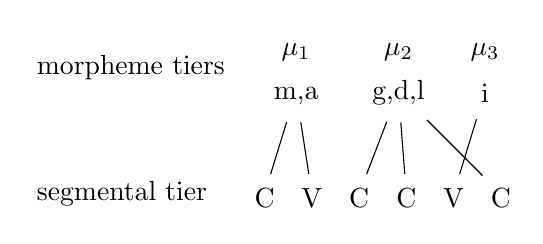
\begin{tikzpicture}[shorten >=2pt,shorten <=3pt, draw=black!100]
	\def \rowthreeht{4.4cm}
	\def \rowtwoht{3.8cm}
	\def \twopointfive{4.1cm}
	%\def \weightstwo{3.75cm}
	\def \rowoneht{2.5cm}
	%\def \weightsone{1.25cm}
	%\def \basement{2cm}
	\tikzstyle{c-node}=[text height=8pt,text centered,inner sep=3pt,minimum size=10pt]
	\tikzstyle{m-node}=[text height=7pt,text centered,inner sep=3pt,minimum size=12pt]
	\tikzstyle{r-node}=[text height=10pt,inner sep=0pt,minimum size=10pt]
	%\tikzstyle{d-node}=[text height=6pt,text centered,inner sep=0pt,minimum size=12pt]
	\tikzstyle{annot}=[text width=25ex,align=left]
	% labels
	\node[annot] (mtierstop) at (0cm,\twopointfive) {morpheme tiers};
	\node[annot] (segtier) at (0cm,\rowoneht) {segmental tier};
	%\node[annot] (mtiersbot) at (0cm,\basement) {};
	
	% surface layer
	\node[r-node] 	(r0)	at (1.0cm,\rowoneht)		{C};
	\node[r-node] 	(r1)	at (1.6cm,\rowoneht)		{V};
	\node[r-node] 	(r2)	at (2.2cm,\rowoneht)		{C};
	\node[r-node] 	(r3)	at (2.8cm,\rowoneht)	 	{C};
	\node[r-node] 	(r4)	at (3.4cm,\rowoneht)	 	{V};
	\node[r-node] 	(r5)	at (4.0cm,\rowoneht)	 	{C};
	
	% hidden-layer elements
	\node[r-node] 	(m0)	at (1.4cm,\rowthreeht)		{$\mu_{1}$};
	\node[r-node] 	(m1)	at (2.7cm,\rowthreeht)		{$\mu_{2}$};
	\node[r-node] 	(m2)	at (3.8cm,\rowthreeht)		{$\mu_{3}$};

	% hidden layer
	\node[c-node] 	(m3)	at (1.4cm,\rowtwoht)		{\/m,a\/};
	\node[c-node] 	(m4)	at (2.7cm,\rowtwoht)		{\/g,d,l\/};
	\node[c-node] 	(m5)	at (3.8cm,\rowtwoht)		{\/i\/};
		
	\path
		(m3)	edge	node	{}	(r0)
		(m3)	edge	node	{}	(r1)
		%
		(m4)	edge	node	{}	(r2)
		(m4)	edge	node	{}	(r3)
		(m4)	edge	node	{}	(r5)
		%
		(m5)	edge	node	{}	(r4);
		
	\end{tikzpicture}
	\label{subfig:nonlinear}
	}

	\subfigure[Linear approach]{
	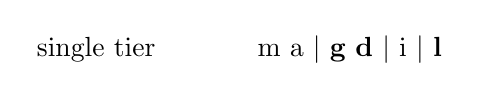
\begin{tikzpicture}[shorten >=1pt,draw=black!100]
	\vspace{50pt}
	\def \floor{0cm}
	\tikzstyle{f-node}=[text centered,inner sep=0pt] %text centered]
	\tikzstyle{annot}=[text width=34ex,align=left]
	% labels
	\node[annot] (floorlabel) at (0cm,\floor) {single tier};
	
	% surface layer
	\node[f-node] 	(f0)	at (1.4cm,\floor)			{m\,\,a\,\,$|$\,\,\textbf{g}\,\,\textbf{d}\,\,$|$\,\,i\,\,$|$\,\,\textbf{l}};
	\end{tikzpicture}
\label{subfig:linear}
}
\caption{Multiple tiers vs. a single tier}
\label{fig:linear}
%\vspace{-20pt}
%\vspace{1pt}
\end{figure}

Notice that $\mu_2$, the consonantal root, is discontinuous; it is
interrupted by $\mu_3$. If a model should have only one tier, as in
fig.~\ref{subfig:linear}, there would be no way of representing the
unity of $\mu_2$, i.e., the fact that \textit{g}, \textit{d}, and \textit{l}
all belong to the same morphological unit. Multiple tiers are thus crucial. With this multi-tier aspect of
autosegmental morphology in mind, we can state two fundamental criteria for any
model of non-concatenative morphology:

\begin{exe}  \ex \label{ex:properties}\begin{xlist}
	\ex {\textsc{Nonlinearity}}: Morphemes are represented as being separate from the segmental tier.
	\ex {\textsc{Nonsequentiality}}: Each morpheme tier (or node) is orthogonal to---i.e., independent of---all other morpheme tiers.
	\end{xlist}
\end{exe}
% \ex this is one 
%\marginpar{or multilinear}
These criteria, or essential properties,
%\textsc{nonlinear} and \textsc{nonsequential} 
are basically binary variables; each \emph{must} be either True or False, and each can \emph{only} be True or False.  Each variable thus has two possible values,
giving us $2^2 = 4$ possible combinations of (non)linearity and (non)sequentiality: 
\textbf{nonlinear nonsequential} (NLNS), \textbf{linear nonsequential} (LNS), 
\textbf{nonlinear sequential} (NLS), and \textbf{linear sequential} (LS).

%[We should note that autosegmental morphology has other properties to
%constrain morphological structure, e.g., the well-formedness
%principle; at present, we are not concerned with capturing all aspects
%of autosegmental morphology, but instead in building a generic system
%to which one can later add linguistically motivated constraints.]

\section{Research objectives}
%State primary research objective: 
\subsection{Primary research objective}
My primary objective is to demonstrate that the multilinear architecture of autosegmental theory can be implemented for the purpose of ULM. That is, my goal is 
to devise \emph{at least one} way of doing this and 
to demonstrate that it works. In particular, I intend to show 
%that the crucial components of autosegmental theory, i.e., 
%those components that allow it to handle non-concatenative morphology, 
that the properties of nonlinearity and nonsequentiality
can be implemented in the form of 
a Multiple Cause Mixture Model (MCMM), 
%which is 
%a general unsupervised learning framework developed by \cite{saund:94}. 
a general unsupervised learning framework developed by \cite{saund:94}. 
I shall thus develop a machine-learning system that is driven by an MCMM.
Its input data will consist of Modern Hebrew words represented as feature vectors. 
I am focusing on Modern Hebrew because 
it exhibits both concatenative and non-concatenative morphological processes 
and thus provides a good test of the method's generality.

\subsection{Secondary research objectives}
\label{sec:secondary-objectives}
My secondary research objectives are outlined below. They are largely concerned with matters of implementation. 
	 \paragraph{Features.} There is a great deal of information tacitly present in a string of alphabetic symbols.
	 This is true regardless of whether the string is written, in which case the symbols are graphemes, or spoken,
	 in which case they are phonemes. In either case, the symbols are each drawn from an alphabet of size $N$ and arranged along a single axis (say, the $x$ axis).
Consider the string of graphemes printed below.
\begin{figure}[h]
	\centering
	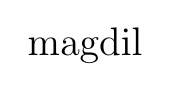
\begin{tikzpicture}[shorten >=2pt,shorten <=3pt, draw=black!100]
	\Large
	\def \rowoneht{0cm}
	\def \rowtwoht{-0.8cm}
	\tikzstyle{r-node}=[text height=10pt,inner sep=0pt,minimum size=10pt]
	%\node[r-node] 	(r0)	at (0cm,\rowoneht)		{\textipa{magdil}};
	\node[r-node] 	(r0)	at (0cm,\rowoneht)		{magdil};
	%\node[r-node] 	(r0)	at (0cm,\rowoneht)		{s t o p};
	%\node[r-node] 	(r0)	at (0cm,\rowtwoht)		{p o t s};
	\end{tikzpicture}
\end{figure}

This row of six graphemes contains a vast amount of tacit information. For instance, suppose we had to represent the string \textit{magdil} not as sequence of alphabetic symbols, but as a series of simple declarative statements. We might come up with statements like the following: 
%These statements might say that a certain character is present in the string, that one character precedes another character, that a particular character occurs at a particular position in the string, and so on, as in the following examples.
\begin{itemize}
  \item \textit{a} immediately follows \textit{m}, \textit{g} immediately follows \textit{a}, \textit{d} immediately follows \textit{g}, and so on. 
  \item \textit{i} immediately precedes \textit{l}, \textit{d} immediately precedes \textit{i}, and so on. %What's more, we know that
   \item \textit{g} follows both \textit{m} and \textit{a}, \textit{d} follows \textit{m}, \textit{a}, and \textit{g}; \textit{d} precedes both \textit{i} and \textit{l}, \textit{g} precedes \textit{d}, \textit{i}, and \textit{l}, and so on.
   \item \textit{m} is the first character, \textit{a} is the second, \dots \textit{i} is the second-to-last character, and \textit{l} is the last character, and so on.
   %\item \textit{l} is the sixth character, \textit{i} is the fifth, \textit{d} is the fourth, and so on.
   \item \textit{m} precedes \textit{a}, \textit{m} precedes \textit{g}, \textit{m} precedes \textit{d}, \dots, \textit{m} precedes \textit{l}; \textit{a} precedes \textit{g}, \dots , \textit{a} precedes \textit{l}; and so on.
   \item \textit{m} is present, \textit{a} is present, \textit{g} is present, and so on.
   \item \emph{ad infinitum}
\end{itemize}
A string of alphabetic symbols tacitly conveys all of these facts and many more---perhaps infinitely more.
Statements like these are essentially what we call \emph{features}.
Each statement can be either true or false, which is to say that each feature is \emph{binary}, drawn from an alphabet of size $N = 2$.  
Many machine learning models require that each input object or \emph{learning instance} (in our case, each \emph{word}) be represented as a vector of binary features, not alphabetic features. Moreover, all input objects (learning instances) must be described by the same feature set, and all feature vectors must be of the same length.

One cannot, of course, have an infinite number of features, as feature vectors must be finite in length.
Now, let $F$ be the infinite set of all possible features. In keeping with the spirit of my primary research objective, we shall assume that there exists at least one $\phi$ such that that $\phi \subset F$, $\phi$ is finite, and $\phi$ allows an ULM system to learn a multilinear model of morphology. The objective here is to confirm this assumption, i.e., to find such a subset.

\paragraph{Data Representation.} The features are extracted from raw-text data, wherein Hebrew words are represented as strings of alphabetic symbols, and the symbols are drawn from a particular alphabet. Now, it so happens that we have more than one alphabet at our disposal, and thus more than one way to represent the input data. These alphabets are the following:
	\begin{enumerate}
		\item \textbf{Modern Hebrew standard orthography}, as transliterated to ASCII characters in the Hebrew Treebank \citep{simaan-et-al:2001}. In the orthography of Modern Hebrew, certain consonants are regularly appropriated to represent vowels. For example, the Hebrew letter
		\textcjheb{w}, transliterated as \textit{w} in the Hebrew Treebank, is by default the consonant /v/, but it is also used to represent the vowels /o/ and /u/. In most syllables, however, the vowel is not represented at all. 
		\item \textbf{Phonemic transcriptions}, i.e., phonemically transcribed words. I have extracted two lists of phonemically transcribed words from the Hebrew portion of the CHILDES database \citep{macwhinney:2000a}. 
		 These lists are the same except that stress is marked in one, but not in the other.
	\end{enumerate}
	%The phonemic transcriptions amount to 12,494 words.
	The question is which mode of representation yields better feature vectors. This is equivalent to asking which mode delivers the largest quantity of useful information and/or the smallest quantity of irrelevant information.
	\paragraph{Mixing and Objective Functions.} The \textbf{mixing function} 
is essentially a voting rule \citep{saund:94}. It prescribes the method whereby the 
``votes" of  hidden units are combined to turn a particular feature (i.e., surface unit) \textsc{on} or \textsc{off} (see section~\ref{sec:mixing-function}. The \textbf{objective function} measures the discrepancy---or, alternatively, similarity---between the surface units' activities and their target activities. 
It thus drives the model's learning by way of trial and error. Objective functions can 
be either positive or negative. Positive objective functions measure similarity and thus 
need to be maximized. Negative objective functions measure error and thus need to be minimized (see section~\ref{sec:mcmm-learning}).

I intend to experiment with two radically different mixing functions, 
viz. one that combines hidden-unit activities linearly and one that combines them nonlinearly.
%(see section~\ref{sec:mixing-function}). 
Similarly, I intend to try out 
%two radically different objective functions, namely 
both a negative and a positive % one (see section~\ref{sec:mcmm-learning}).
objective function. %(see section~\ref{sec:mcmm-learning}).
%Why: What does the mixing function do? What would happen if there were no mixing function? The mixing function maps the hidden-unit activities
%What does the objective function do? What would happen if there were no objective function? 
%If there were no objective function, there could be no learning. Learning proceeds by trial and error. 
%The objective function supplies the error.

\paragraph{Evaluation.} The system described in this proposal is an unsupervised learning system and is thus inherently difficult to evaluate, as one goal of unsupervised learning is to discover previously unknown categories \citep{parsons:2004}.
The previously unknown categories in this case are going to be morphological units of some kind.
However, these units will not be conventional morphemes or morphosyntactic categories. 

Instead, MCMM-generated clusters will correspond roughly to Aronoff's 
\emph{morphomes} \citep{aronoff:1994}, which can be described as \emph{pre-morphosyntactic} units, i.e.,
units that have been assembled from phonemes, but have not yet been assigned 
a syntactic or semantic meaning. I shall use the term \emph{morph} instead of 
\emph{morphome}, however, since MCMM-generated clusters may not correspond 
precisely to morphomes in every case (see section~\ref{sec:targets}).

Thus, the evaluation itself presents an important research question, namely the question of how to evaluate the output of an unsupervised morphological clustering algorithm, particularly one that considers only features of \emph{word-internal form}, having no access to word-external morphosyntactic features, e.g., the person, number, and gender of  surrounding words.

%Thus, my system will not require morphological building blocks to have particular
%meanings. Instead, it 
%My system will thus look for \emph{pre-morphosyntactic} 
%units, i.e., ones assembled from phonemes, but not yet assigned 
%a syntactic or semantic meaning. In a larger pipeline, such 
%building blocks could serve as an interface between morphosyntax 
%and phonology. For instance, while an MCMM can find Hebrew's default 
%masculine suffix \textit{-im}, it cannot say whether it is
%masculine or feminine in a given word, as this suffix
%also occurs in idiosyncratic feminine plurals. The extrinsic part of the evaluation will examine my system's utility as a component within such a pipeline
%(see section~\ref{sec:paradigms}).
%\emph{morphs}. \marginpar{I have yet to introduce morphs, tho} We do not know 
%beforehand \emph{exactly} what these morphs ought to look like. Since we cannot know 
%the ``right answers" before the experiments are run, there can be no clear gold 
%standard against which to evaluate the MCMM's output. 
%
%Thus, the evaluation itself presents an important research question, namely the question of how to evaluate the output of an unsupervised morphological clustering algorithm, particularly one that considers only features of \emph{word-internal form}, having no access to word-external morphosyntactic features, e.g., the person, number, and gender of  surrounding words. Such an algorithm will inevitably produce clusters that do not correspond to abstract morphosyntactic categories or conventional morphemes.
%which are fundamentally morphosyntactic in nature even though the correspondence between morphemes and abstract, or ``atomic," morphosyntactic categories is not always one-to-one.
